% Begin a new LaTeX document.
\documentclass[convert={density=300,size=1080x800,outext=.png}]{standalone}


% Include the necessary packages for drawing the flow diagram.
\usepackage{tikz}
\usetikzlibrary{decorations.pathmorphing, patterns}
\usepackage{xcolor}
\definecolor{myblue}{RGB}{62,146,255}
\definecolor{myred}{RGB}{228,3,43}

\begin{document}


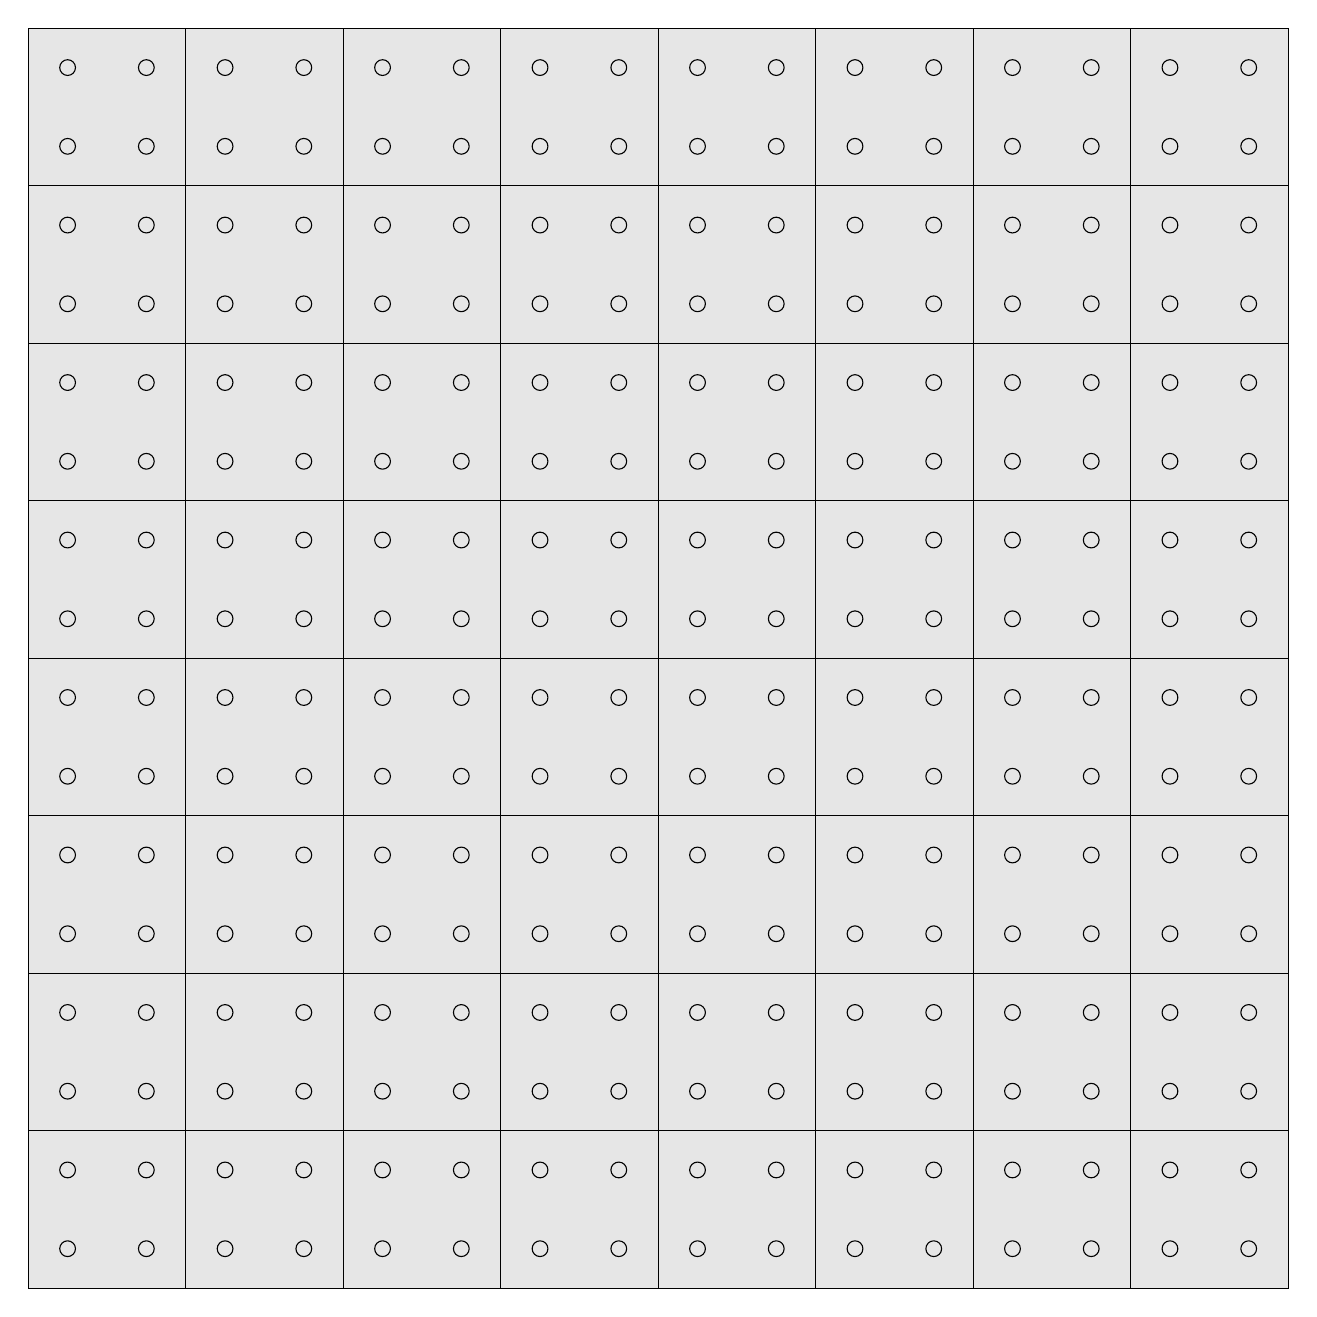
\begin{tikzpicture}[>=latex]
  \def\Ncell{16}
  
  \def\incl{2}
  \pgfmathsetmacro\I{0.5/\incl}
  \pgfmathsetmacro\N{\Ncell/\incl}
  \def\r{0.1}

  \fill[gray, fill opacity=0.2, draw = black] (0,0) rectangle (\Ncell,\Ncell);
  \foreach \x in {1, ..., \N} {
      \draw[black] (\x * \incl, 0) -- (\x * \incl, \Ncell);
      \draw[black] (0, \x * \incl) -- (\Ncell, \x * \incl);
  }
  % inclusions
  \foreach \i in {1, ..., \Ncell} {
    \foreach \j in {1, ..., \Ncell} {
          \draw[] (-0.5+\i,-0.5+\j) circle (\r);
    }
  
  }
\end{tikzpicture}
\end{document}